\subsection{Aktorik und Sensorik}
Der folgenden Abschnitt beschreibt die verwendeten elektrischen Bauteile, um einerseits die benötigten physikalischen Größen zu messen, und andererseits die verwendete Aktorik, um das Aufspringen und Balancieren der Würfelseite zu ermöglichen.
\newline 

Die Aufgabe der Sensorik besteht darin die Zustandsgrößen des Systemes zu bestimmen. Hierfür werden zwei \textit{GYR-521}-Platinen verwendet, die mit einem \textit{MPU6050}-IC der Firma \textit{InvenSense} bestückt sind. Diese bieten jeweils einen dreiachsigen Beschleunigungssensor und Gyroskop. Mit Hilfe dieser Messwerte können die Zustandsgrößen $\varphi$ und $\dot{\varphi}$ berechnet werden. Die Sensoren bieten die zusätzliche Möglichkeit einen variablen Tiefpassfilter zu verwenden um eine erste Glättung der Messwerte durchzuführen. Dieses Tiefpassfilter wird auf eine Grenzfrequenz von $44Hz$ eingestellt. Dieser Wert hat sich empirisch als optimaler Kompromiss zwischen Filterung der Rauschsignale und Verzögerung des eigentlichen Signals ergeben. Die Konfiguration und Auswertung der Sensoren erfolgt über eine $I^2C$-Schnittstelle. Die Justierung und Auswertung der Sensoren wird näher in Abschnitt \ref{sensorik_sec} beschrieben.
\newline

Abschnitt \ref{Dynamik_sec} zeigt den Einfluss eines Motormomentes auf die Position und Gewschwindigkeit der Würfelseite. Um diese Moment zu erzeugen wird ein bürstenloser DC-Motor der Firma \textit{MaxonMotor} verwendet (EC 45 flat, 50 Watt). Die Kriterien zur Auswahl des Motors sind einerseits die maximale Drehzahl und Drehmoment, andererseits die mechanische Zeitkonstante. Für das Aufspringen des Würfels ist die maximale Drehzahl des Motors von Bedeutung, die 10000 Umdrehung pro Minute des gewählten Motor reichen hierbei aus um eine ausreichend hohe kinetische Energie der Schwungmasse zu ermöglichen. Die Robustheit der Regelung wird durch das maximale Drehmoment limitiert, welches in diesem Fall bei 83.4 mNm liegt. Von besondere Bedeutung für die Regelung ist die mechanische Zeitkonstante des Motors, da diese eine Verzögerung der Stellgröße bewirkt und somit den geschlossenen Regelkreis negativ beeinflussen kann. Die mechanische Zeitkonstante des gewählten Motors ist mit $13.3ms$ im Vergleich zu anderen Kandidaten sehr niedrig. Die Ansteuerung des Motors erfolgt über den Treiberbaustein \textit{ESCON 36/3 EC}, welcher ebenfalls von der Firma \textit{MaxonMotor} vertrieben wird. Dieser ermöglicht die Steuerung des Drehmoments über ein PWM-Signal und die Auswertung der Winkelgeschwindigkeit $\dot{\psi}$ über ein analoges Signal.
\newline

Mit Hilfe einer mechanischen Bremse kann die Schwungmasse stoßartig zum Stillstand gebracht werden. Dadurch wird die kinetische Energie der Schwungmasse teilweise auf das Gesamtsystem übertragen und ermöglicht somit das Aufspringen. Die Bremsbacken werden über einen Servomotor betätigt, welcher mit Hilfe eines PWM-Signales kontrolliert wird.
\newline

Zur Ansteuerung der Aktorik und Sensorik wird ein BeagleBone Black verwendet, auf welchem eine Linux-Distribution ausgeführt wird. Die Programmierung erfolgt über eine, auf Eclipse basierende, Toolkette. Um die Auswertung der Sensordaten und den Entwurf der Regelung zu erleichtern, werden Sensoren- und Regelungsdaten an MATLAB übertragen, wo weitere Auswertungen stattfinden.


\begin{figure}[!h]
\centering
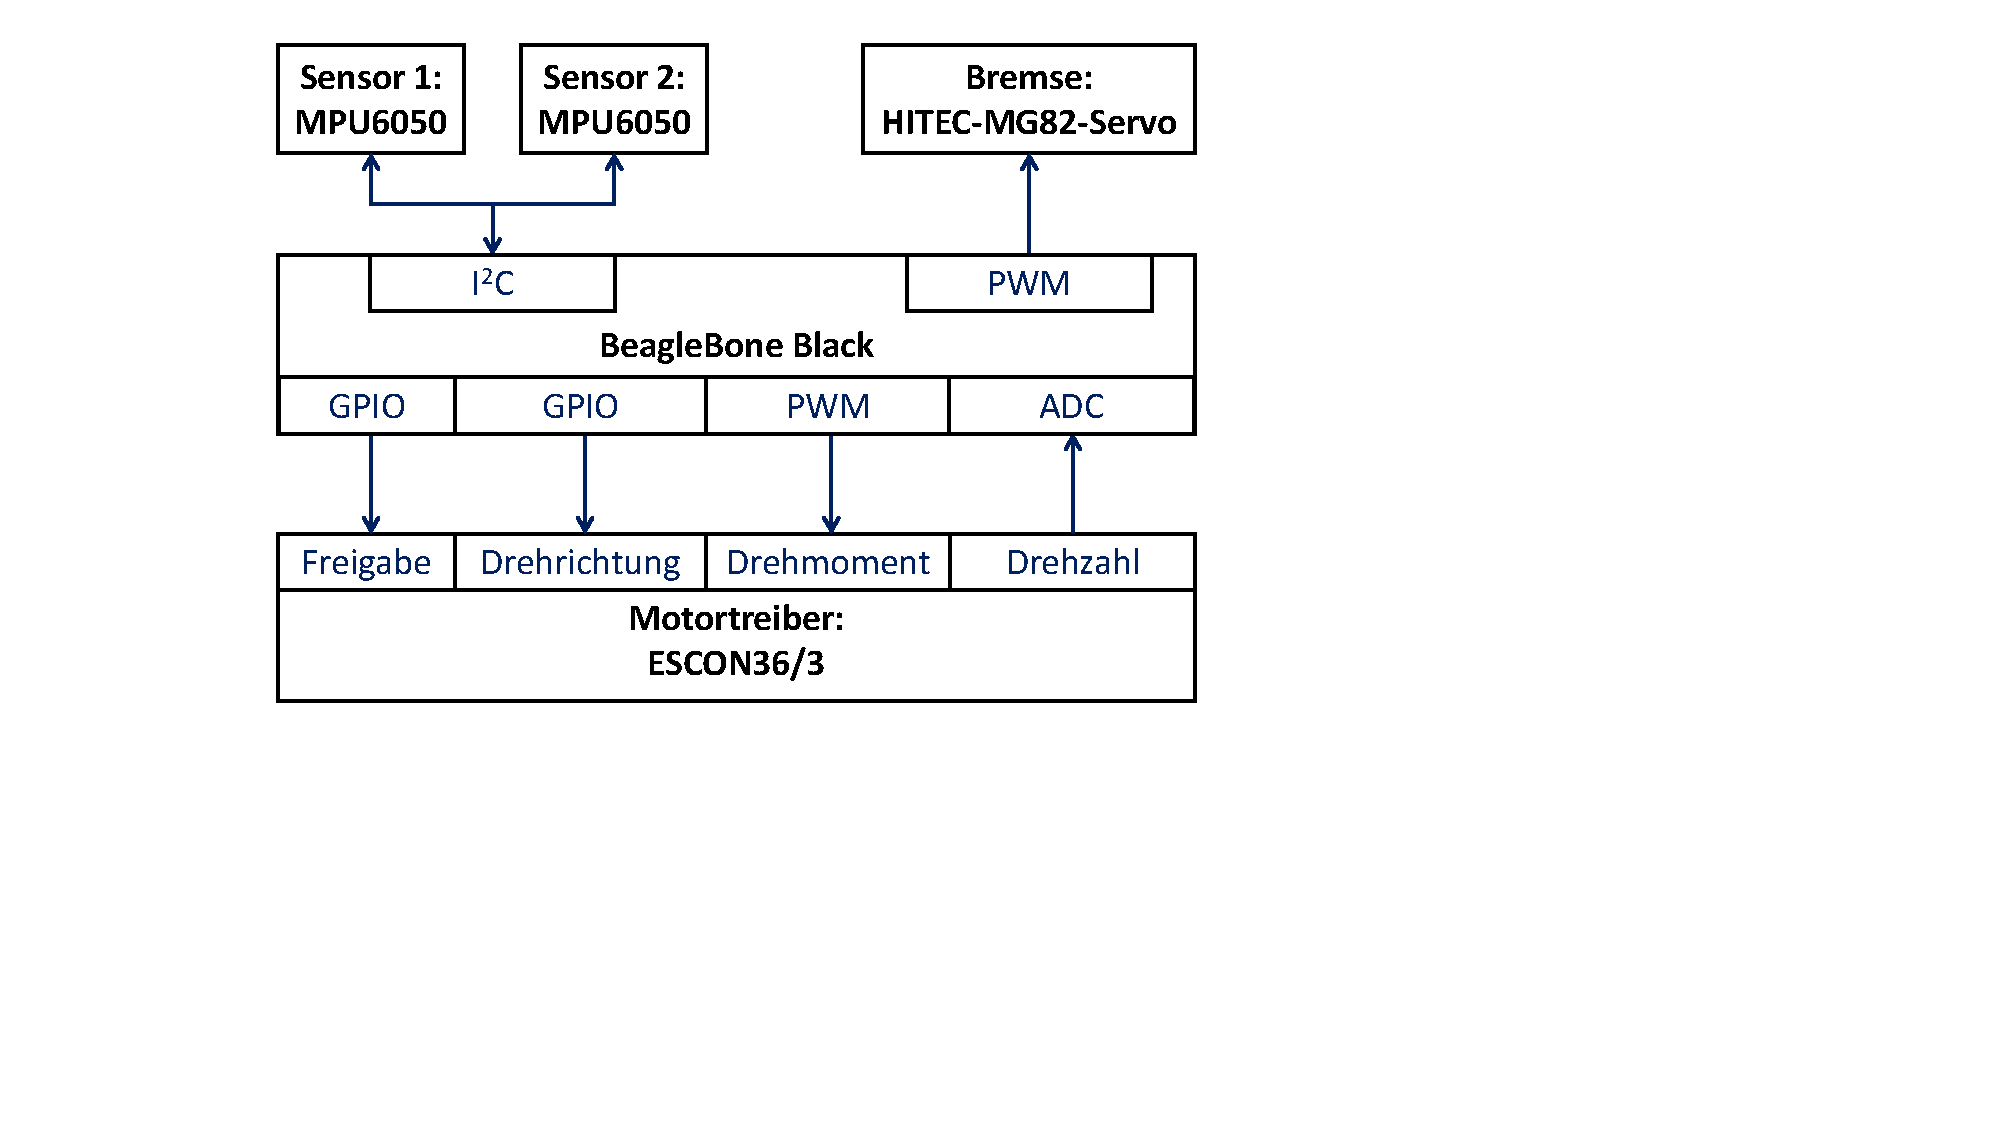
\includegraphics[width=0.7\linewidth, trim={2cm 7cm 11cm 0cm},clip]{img/ElekAufbau_Bauteile}
\caption{Übersicht Elektrik, Quelle: eigene Darstellung}

\end{figure}